
%(BEGIN_QUESTION)
% Copyright 2011, Tony R. Kuphaldt, released under the Creative Commons Attribution License (v 1.0)
% This means you may do almost anything with this work of mine, so long as you give me proper credit

A DP transmitter is used to measure the flow of steam through a venturi tube:

$$\includegraphics[width=15.5cm]{i01275x01.eps}$$

Identify the correct positions for the four hand valves labeled in the diagram during normal operation.  Simply mark the appropriate boxes in the table to answer this portion of the question:

% No blank lines allowed between lines of an \halign structure!
% I use comments (%) instead, so that TeX doesn't choke.

$$\vbox{\offinterlineskip
\halign{\strut
\vrule \quad\hfil # \ \hfil & 
\vrule \quad\hfil # \ \hfil & 
\vrule \quad\hfil # \ \hfil \vrule \cr
\noalign{\hrule}
%
% First row
Valve & Open & Shut \cr
%
\noalign{\hrule}
%
% Another row
V1 &   & \cr
%
\noalign{\hrule}
%
% Another row
V2 &   & \cr
%
\noalign{\hrule}
%
% Another row
V3 &   & \cr
%
\noalign{\hrule}
%
% Another row
V4 &   & \cr
%
\noalign{\hrule}
} % End of \halign 
}$$ % End of \vbox

Next, suppose operations personnel suspected this flow transmitter to be in error, and noted that it had been several years since the transmitter was last calibrated.  Explain how you could check the calibration of this transmitter, particularly how you could tell whether the miscalibration resided in the {\it sensor trim} (ADC) or {\it output trim} (DAC) of the transmitter, using a HART communicator as your {\it only} piece of test equipment.  Note: your answer needs to explain how to {\it check} for the presence of a calibration error, not how to {\it correct} a calibration error, specifically identifying parameters you would monitor using the HART communicator!

\vskip 50pt

\underbar{file i01275}
%(END_QUESTION)





%(BEGIN_ANSWER)

% No blank lines allowed between lines of an \halign structure!
% I use comments (%) instead, so that TeX doesn't choke.

$$\vbox{\offinterlineskip
\halign{\strut
\vrule \quad\hfil # \ \hfil & 
\vrule \quad\hfil # \ \hfil & 
\vrule \quad\hfil # \ \hfil \vrule \cr
\noalign{\hrule}
%
% First row
Valve & Open & Shut \cr
%
\noalign{\hrule}
%
% Another row
V1 &  & $\surd$ \cr
%
\noalign{\hrule}
%
% Another row
V2 & $\surd$ &  \cr
%
\noalign{\hrule}
%
% Another row
V3 &  & $\surd$\cr
%
\noalign{\hrule}
%
% Another row
V4 & $\surd$ &  \cr
%
\noalign{\hrule}
} % End of \halign 
}$$ % End of \vbox

\vskip 10pt

Block and equalize the transmitter using the 3-valve manifold, then check to see that the communicator shows a zero pressure value for {\tt PV} -- this will check for a sensor trim error.  If there is no sensor trim error, the only remaining calibration error in the transmitter must be an output trim error.

Note that checking for correspondence between the displayed {\tt PV} and {\tt AO} values shown by the communicator does {\it nothing} to check either a sensor or an output calibration error.  The displayed AO value will properly correspond with the displayed PV value even if the sensor and/or DAC are grossly miscalibrated!

\vskip 10pt

One point each for the valve positions, 6 points for correct explanation.

%(END_ANSWER)





%(BEGIN_NOTES)

{\bf This question is intended for exams only and not worksheets!}.

%(END_NOTES)

